%% This is an example first chapter.  You should put chapter/appendix that you
%% write into a separate file, and add a line \include{yourfilename} to
%% main.tex, where `yourfilename.tex' is the name of the chapter/appendix file.
%% You can process specific files by typing their names in at the 
%% \files=
%% prompt when you run the file main.tex through LaTeX.
\chapter{Introduction}

\section{Motivations}

\begin {figure}[htbp]
\centering

\includegraphics[width=\textwidth]{scottcaan1}
\caption{Scott Caan}
\label{fig1}
\centering
\end{figure}
\subsection{Specific aim 1: Scott Caan }

        	Scott Caan, scott caan scott caan scott caan? Scott "caan" scott caan scott "caan": scott caan, scott caan scott, caan scott caan scott. Scott caan scott.
\subsection{Specific Aim 2: Scott Caan}

Scott caan scott caan scott caan. Scott "caan", scott caan scott\cite{caan1}, caan scott, caan scott.
 
\begin {figure}[htbp]
\centering
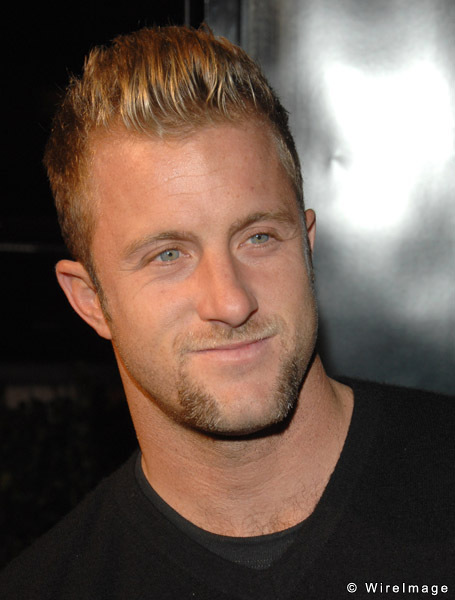
\includegraphics[scale=.5]{scottcaan2}
\caption{Scott Caan}
\label{fig2}
\centering
\end{figure}

 
\subsection {Specific aim 3: Scott Caan}

Scott caan, scott caan scott, caan\cite{caan2} "scott caan", scott caan. Scott caan; scott, caan, scott, caan scott. 

\section{Innovation}
Scott caan? Scott caan.
\begin {figure}[htbp]
\centering

\includegraphics[scale=0.5]{scottcaan3}
\caption{Scott Caan}
\label{fig3}
\centering
\end{figure}

\section{Background}

\subsection{Scott Caan}
	Scott caan scott. Scott caan scott caan scott: caan scott caan.
\subsection{Scott Caan}
	Scott caan scott? Caan scott caan scott. Caan scott caan scott, caan scott. 
\begin {figure}[htbp]
\centering

\includegraphics[scale=.5]{scottcaan4}
\caption{Scott Caan}
\label{fig4}
\centering
\end{figure}

Scott caan scott caan scott caan scott, caan scott caan.\cite{caan3} "Scott Caan", scott caan scott caan. Scott Caan.
 

\subsection{Abbreviations}
\textbf{SC} Scott Caan
